\documentclass[12pt,a4]{article}
\usepackage[]{graphicx}\usepackage[]{xcolor}
% maxwidth is the original width if it is less than linewidth
% otherwise use linewidth (to make sure the graphics do not exceed the margin)
\makeatletter
\def\maxwidth{ %
  \ifdim\Gin@nat@width>\linewidth
    \linewidth
  \else
    \Gin@nat@width
  \fi
}
\makeatother

\definecolor{fgcolor}{rgb}{0.345, 0.345, 0.345}
\newcommand{\hlnum}[1]{\textcolor[rgb]{0.686,0.059,0.569}{#1}}%
\newcommand{\hlstr}[1]{\textcolor[rgb]{0.192,0.494,0.8}{#1}}%
\newcommand{\hlcom}[1]{\textcolor[rgb]{0.678,0.584,0.686}{\textit{#1}}}%
\newcommand{\hlopt}[1]{\textcolor[rgb]{0,0,0}{#1}}%
\newcommand{\hlstd}[1]{\textcolor[rgb]{0.345,0.345,0.345}{#1}}%
\newcommand{\hlkwa}[1]{\textcolor[rgb]{0.161,0.373,0.58}{\textbf{#1}}}%
\newcommand{\hlkwb}[1]{\textcolor[rgb]{0.69,0.353,0.396}{#1}}%
\newcommand{\hlkwc}[1]{\textcolor[rgb]{0.333,0.667,0.333}{#1}}%
\newcommand{\hlkwd}[1]{\textcolor[rgb]{0.737,0.353,0.396}{\textbf{#1}}}%
\let\hlipl\hlkwb

\usepackage{framed}
\makeatletter
\newenvironment{kframe}{%
 \def\at@end@of@kframe{}%
 \ifinner\ifhmode%
  \def\at@end@of@kframe{\end{minipage}}%
  \begin{minipage}{\columnwidth}%
 \fi\fi%
 \def\FrameCommand##1{\hskip\@totalleftmargin \hskip-\fboxsep
 \colorbox{shadecolor}{##1}\hskip-\fboxsep
     % There is no \\@totalrightmargin, so:
     \hskip-\linewidth \hskip-\@totalleftmargin \hskip\columnwidth}%
 \MakeFramed {\advance\hsize-\width
   \@totalleftmargin\z@ \linewidth\hsize
   \@setminipage}}%
 {\par\unskip\endMakeFramed%
 \at@end@of@kframe}
\makeatother

\definecolor{shadecolor}{rgb}{.97, .97, .97}
\definecolor{messagecolor}{rgb}{0, 0, 0}
\definecolor{warningcolor}{rgb}{1, 0, 1}
\definecolor{errorcolor}{rgb}{1, 0, 0}
\newenvironment{knitrout}{}{} % an empty environment to be redefined in TeX

\usepackage{alltt}
\newcommand{\SweaveOpts}[1]{}  % do not interfere with LaTeX
\newcommand{\SweaveInput}[1]{} % because they are not real TeX commands
\newcommand{\Sexpr}[1]{}       % will only be parsed by R



% ---- Metadata ---- %

\title{Honesty by Convenience: Corruption Tolerance in Ecuador}
\author{Daniel Hernán Sánchez Pazmiño}
\date{June 2022}

% ---- Load Packages ---- %

% Math

\usepackage{savesym} % Need to "save" the command that is already defined \varTheta

\usepackage{amsmath}
  \savesymbol{varTheta} 

% Fonts

% To set the TNR font for both text and equations:

\usepackage{mathspec}
  \setallmainfonts(Digits,Greek,Latin){Times New Roman}
\restoresymbol{MTP}{varTheta}

% Formatting

\usepackage{setspace}
  \doublespacing

\usepackage[margin = 1in]{geometry}

\usepackage{lscape}

% Citation & Bibliographies

\usepackage[backend = biber, style = apa, citestyle = apa]{biblatex}
  \addbibresource{refs.bib}
  
% For tables:

 % For the modelsummary tables:
\usepackage{siunitx}
\usepackage{booktabs} 
  \newcolumntype{d}{S[input-symbols = ()]}

\usepackage{caption}
\usepackage{multirow}
\usepackage[flushleft]{threeparttable}
  
% Other packages

\usepackage{csquotes} % For quotation marks

\usepackage{epigraph} % For epigraph
  \setlength\epigraphwidth{9cm}
  \setlength\epigraphrule{1pt}

\usepackage{float} % For the H float option- only used in emergencies (lol)

\usepackage{textcomp} % For the registered trademark symbol.

% Always load these packages at the end of the preamble:

\usepackage{hyperref}

% ---- R Stuff to be used in the whole document ----

% Here I will execute or source R code through chunks that I need to use throughout the whole document.

% General settings



% Load the data by sourcing the data manipulation script. Note that survey design objects are indeed created in this script.




\begin{document}
% Results II .Rnw File

\subsection{Baseline regressions}
\label{subsec:fin2}

Based on the previous subsection's findings, some potential key determinants for corruption tolerance are considered. Two economic variables at the individual level significantly changed during this period: the percent of people who report a worse economic situation as well as the indicator of unemployment. These follow macroeconomic indicators for the Ecuadorian economy too, as can be seen in Figure \ref{fig:ecua_ec}. Variables which proxy attitudes in the political landscape also have significantly changed: the percentage of people who confide in the President, the percentage who approve the President's job and also the percentage of people who identify with the political right wing.

Simple empirical models are estimated to study the relationship of these key changes with corruption tolerance, which follow the equation below:
\begin{equation}
\label{eqn:simplemod}
P(ctol = 1 | \textbf{\textit{X}} \hspace{0.04cm}) = G \left[ \beta_0 + \delta_0 y_{16} + \beta_1 x^* + \delta_1 (y_{16} \cdot x^*) + u\right]
\end{equation}
where $x^*$ is the key regressor, which can either be: 
\begin{itemize}
  \item A dummy variable set to unity for respondents who answered that their economic situation is worse (Model 1)
  \item A dummy variable set to unity for respondents who report being unemployed (Model 2)
  \item A discrete variable with numbers 1-7, where higher numbers imply a higher degree of confidence in the President (Model 3)
  \item A discrete variable with numbers 1-5, with higher numbers implying a higher rating of the President's job performance (Model 4)
  \item A discrete variable with numbers from 1-10 where 1 is the extreme left and 10 is the extreme right (Model 5)
\end{itemize}
% Now I'm going to run the first models, and I'll do so by sourcing a script.


% Now, I'll make the table with modelsummary from the sourced stuff. 
\begin{table}[htbp]
\caption{Logit coefficients for baseline models}
\label{tab:simplemodel}

\begin{tabular}[t]{lccccc}
\toprule
  & Model 1 & Model 2 & Model 3 & Model 4 & Model 5\\
\midrule
Constant & \num{-1.894}*** & \num{-1.989}*** & \num{-0.455}** & \num{0.553} & \num{-1.527}***\\
 & (\num{0.127}) & (\num{0.110}) & (\num{0.208}) & (\num{0.362}) & (\num{0.196})\\
2016 Dummy & \num{0.848}*** & \num{1.001}*** & \num{-0.188} & \num{-1.251}*** & \num{0.278}\\
 & (\num{0.158}) & (\num{0.132}) & (\num{0.238}) & (\num{0.415}) & (\num{0.234})\\
Worse Economic Situation & \num{0.131} &  &  &  & \\
 & (\num{0.169}) &  &  &  & \\
Unemployment &  & \num{1.015}*** &  &  & \\
 &  & (\num{0.205}) &  &  & \\
Confidence in President &  &  & \num{-0.288}*** &  & \\
 &  &  & (\num{0.037}) &  & \\
Approval of Pres. Performance &  &  &  & \num{-0.648}*** & \\
 &  &  &  & (\num{0.096}) & \\
Political Wing &  &  &  &  & \num{-0.047}\\
 &  &  &  &  & (\num{0.038})\\
Econ. Situation Interaction & \num{-0.025} &  &  &  & \\
 & (\num{0.197}) &  &  &  & \\
Unemployment Interaction &  & \num{-1.005}*** &  &  & \\
 &  & (\num{0.256}) &  &  & \\
Pres. Confidence Interaction &  &  & \num{0.206}*** &  & \\
 &  &  & (\num{0.044}) &  & \\
Pres. Approval Interaction &  &  &  & \num{0.568}*** & \\
 &  &  &  & (\num{0.111}) & \\
Pol. Wing Interaction &  &  &  &  & \num{0.095}**\\
 &  &  &  &  & (\num{0.043})\\
\midrule
$N$ & \num{2948} & \num{2950} & \num{2944} & \num{2941} & \num{2535}\\
AIC & \num{2893.64} & \num{2889.04} & \num{2848.57} & \num{2844.82} & \num{2574.81}\\
BIC & \num{2926.37} & \num{2920.98} & \num{2881.80} & \num{2876.65} & \num{2606.10}\\
\bottomrule
\end{tabular}


\vspace{0.25cm}
\textbf{Note:} Logit coefficients of the baseline models as described by Equation \ref{eqn:simplemod}. Standard errors consider design effects of the AB complex survey design.\\
*$p$ < 0.1, **$p$< 0.05, ***$p$ < 0.01.
\end{table}

Table \ref{tab:simplemodel} presents the logit estimates of the model coefficients for Equation \ref{eqn:simplemod}. The coefficient for the year dummy shows the significance of the jump in corruption tolerance for year 2016. This significance is lost when considering interaction terms with confidence in the President. The year dummy actually has a negative sign when the approval of his job performance and the political score variable are considered. While unemployment does seem to have a significant effect in year 2014 and also in an interaction term, its inclusion does not eliminate the significance of the year dummy. The coefficients also suggest that a person who reports having a worse economic situation does not tolerate corruption more or less than those who report a same or equal economic situation. 

Model 1 suggests that a person who reports having a worse economic situation does not tolerate corruption differently than those who report a same or higher economic situation. Model 2 shows that respondents who were unemployed were more likely to justify corruption than those who were not unemployed (either employed or not in the labor force, see \hyperref[app:first]{Appendix A}). The interaction term in this model has a negative sign, which shows that the effect of unemployment in 2016 was less than the effect in 2014. While this relationship would not clearly explain the jump in corruption tolerance, it is an interesting finding which will be explored further. 

Models 3 and 4 display the same relationship: people who either trust or approve of the President in a higher degree also tolerate corruption less. A more zealous supporter of the regime will believe that bribes are not justified given the actual situation, however, this appears to change in 2016. The interaction term for both variables are significant and positive: in 2016 regime supporters started to justify corruption in a higher degree relative to 2014 levels. This could explain the jump in corruption tolerance since support for the President eroded in 2016, which meant that the number of non-supporters was higher; these respondents justified corruption more than supporters. Also, the supporters that remained started to justify bribes to a higher degree for this year. In Model 3, the significance of the year dummy is lost, while in Model 4 its sign is reversed.

The political identification of respondents is taken into account in Model 5. The coefficients show that a person who identifies closer to the political right does not justify corruption differently relative to people identifying closer to the political left. However, the interaction term shows that people answering higher values of this variable justified corruption more in 2016. Once again, the significance of the year dummy is lost when considering this variable. With a higher number of respondents identifying with the political right wing, who appear to justify corruption more, it would be understood how overall corruption tolerance increased. This estimate, however, is less statistically significant than the other three interaction terms in the other models. 

All of these results hold with the logit and linear probability models, which can be seen in Appendix \label{app:second}. Table \ref{tab:apebase} presents average partial effects for the model estimations in Table \ref{tab:simplemodel}. Table \ref{tab:apesimp} presents average partial effects for the five models of Table \ref{tab:simplemodel}. These figures show that an unemployed person is 5.9\% more likely to justify corruption. Additionally, a respondent who answered one number higher for an increased degree of confidence in the President was 2.4\% less likely to justify corruption. Finally, a person who rated the President's job performance one unit higher was 4.4\% less likely to justify corruption. All other partial effects are not significant. Similar magnitudes are obtained for the probit model average partial effects, as seen in Table \ref{tab:probitsimpape}. 

% Do the APE table (pending)

% I need to draw the graph which shows the visual differences between groups and their corruption tolerance

% I draw my data by sourcing the tabulations script.



% Now I do the data wrangling needed for this


% Now do the graph
\begin{figure}[htbp]
\caption{Graphical representations of corruption tolerance across key explanatory variables}
\label{fig:difgraph}
\fbox{
\begin{minipage}{\textwidth}
\begin{knitrout}
\definecolor{shadecolor}{rgb}{0.969, 0.969, 0.969}\color{fgcolor}

{\centering 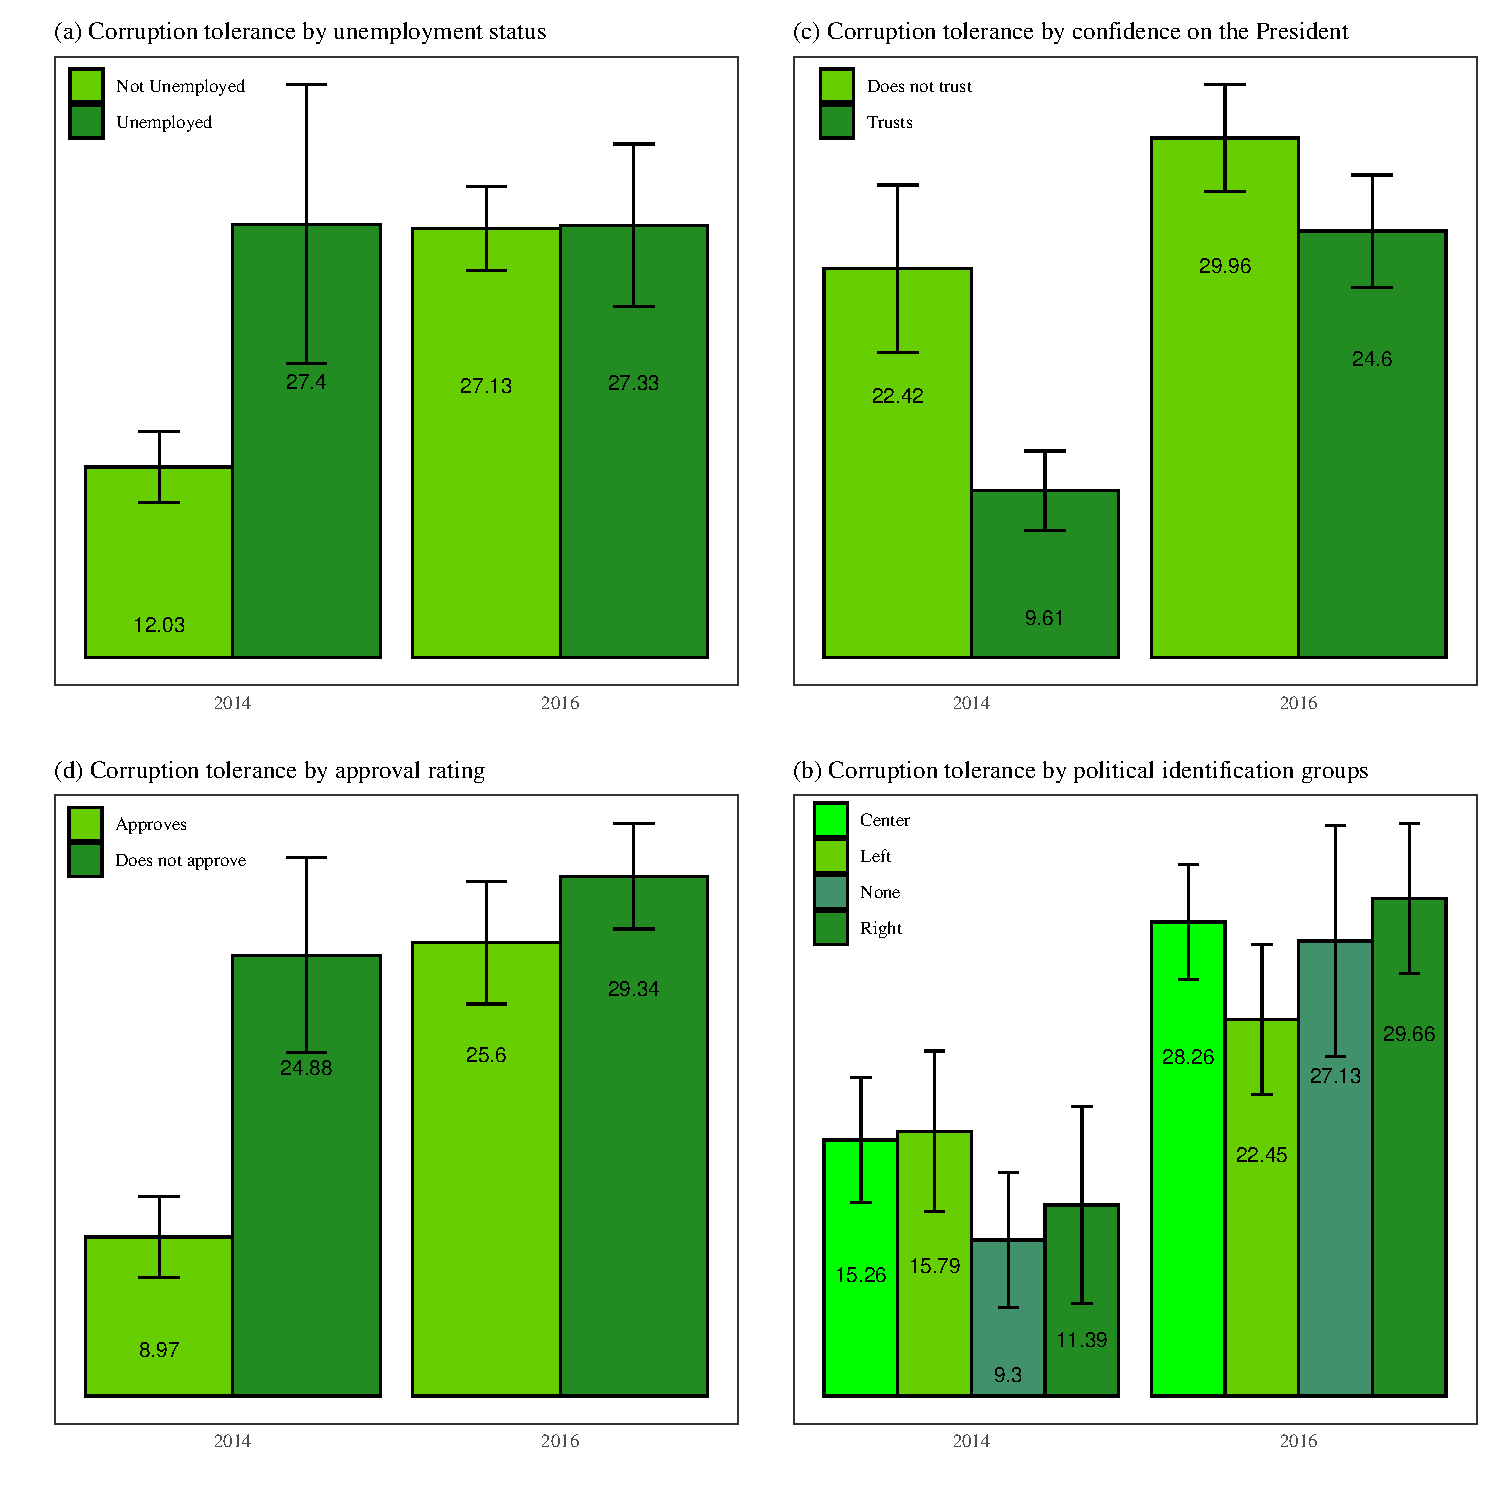
\includegraphics[width=\maxwidth]{figure/difgraph-1} 

}


\end{knitrout}
\textbf{Note:} Figures show the percent of respondents that justify corruption across the groups used as explanatory models in Table \ref{tab:simplemodel}. Data from the open-access databases of the AB. Error bars represent the 95\% confidence intervals considering design effects. Figure prepared by the author. 
\end{minipage}
}
\end{figure}

The findings of these models can be further explained by Figure \ref{fig:difgraph}. According to panel (a), in 2014, only 12.03\% of people who were not unemployed justified corruption, while in 2016 this figure increased to 27.03\%, very close to the percentage of unemployed people who justified it in 2016. The difference between time periods of these percentages is not statistically significant, which means that in 2016 the effect of unemployment in corruption tolerance approached zero. Thus, Figure \ref{fig:difgraph} along with Model 2 of Table \ref{tab:simplemodel} show that it was not the unemployed who started to justify corruption less, it was that the people who were not unemployed started to justify it more. Panels (b) and (c) of Figure \ref{fig:difgraph} show that the percentage of people who either confided in or approved the President and justified corruption increased significantly  between 2014 and 2016. This means that the negative effect of supporting the executive in 2016 was smaller than in 2014, as confirmed by the interaction term in Models 3 and 4 of Table \ref{tab:simplemodel}. In panel (d) of Figure \ref{fig:difgraph}, where four different political groups are considered: the left, right, center and those who did not answer the question. All four groups saw increases in the percent of group members who justify corruption. All increases in corruption tolerance are significant, except for those who identify with the left wing. This is consistent with the coefficient sign seen in Model 5 for the political score variable. 



\end{document}
